% ============================================================
%  MAIN.TEX – Tệp gốc báo cáo
%  Gaussian Mixture Model và Thuật toán Expectation-Maximization
% ============================================================
\documentclass[12pt, a4paper]{article}

\input{preamble}

% ============================================================
%  Thông tin tài liệu
% ============================================================
\hypersetup{
  pdftitle  = {Mô hình Hỗn hợp Gaussian và Thuật toán EM},
  pdfauthor = {Nhóm sinh viên},
  pdfsubject= {Toán cho Khoa học Máy tính},
}

% ============================================================
\begin{document}
% ============================================================

% ------------------------------------------------------------
%  Trang bìa
% ------------------------------------------------------------
\begin{titlepage}
  \centering
  \vspace*{1cm}

  {\Large\bfseries TRƯỜNG ĐẠI HỌC CÔNG NGHỆ THÔNG TIN \ldots\\[4pt]
   KHOA KHOA HỌC MÁY TÍNH \ldots}

  \vspace{1.5cm}
  \rule{\linewidth}{1.5pt}\\[6pt]
  {\LARGE\bfseries Mô hình Hỗn hợp Gaussian\\[6pt]
   và Thuật toán Expectation-Maximization}\\[6pt]
  \rule{\linewidth}{1.5pt}

  \vspace{1cm}
  {\large Báo cáo môn: \textbf{Toán cho Khoa học Máy tính}}

  \vspace{2cm}
  \begin{tabular}{ll}
    \textbf{Nhóm thực hiện:} & \\[4pt]
    \quad Nguyễn Phúc Thuận & -- MSSV: 25521820 \\
    \quad Huỳnh Ngọc Phước Thịnh & -- MSSV: xxxxxx \\
    \quad Họ tên thành viên 3 & -- MSSV: xxxxxxxx \\
    \quad Họ tên thành viên 4 & -- MSSV: xxxxxxxx \\[8pt]
    \textbf{Giảng viên hướng dẫn:} & Thầy/Cô \ldots \\[8pt]
    \textbf{Học kỳ:}  & \ldots -- Năm học: 20xx--20xx \\
  \end{tabular}

  \vfill
  {\large Thành phố Hồ Chí Minh, tháng~\ldots~năm~20xx}
\end{titlepage}

% ------------------------------------------------------------
%  Tóm tắt
% ------------------------------------------------------------
\begin{abstract}
  \noindent
  Báo cáo này trình bày lý thuyết và ứng dụng của Mô hình Hỗn hợp Gaussian
  (Gaussian Mixture Model – GMM) và thuật toán Expectation-Maximization (EM).
  Chúng tôi bắt đầu từ nền tảng toán học cần thiết, xây dựng mô hình GMM,
  suy dẫn đầy đủ các bước E-step và M-step, phân tích tính hội tụ, rồi so sánh
  GMM với phương pháp phân cụm $k$-means.
  Phần thực nghiệm minh họa hoạt động của thuật toán trên các bộ dữ liệu tổng hợp
  và thực tế, kèm theo phân tích định lượng.

  \medskip\noindent
  \textbf{Từ khóa:} Mô hình hỗn hợp Gaussian, Thuật toán EM,
  Phân cụm mềm, Biến ẩn, Hội tụ log-likelihood.
\end{abstract}

% ------------------------------------------------------------
%  Mục lục & danh sách hình/bảng
% ------------------------------------------------------------
\tableofcontents
\clearpage
\listoffigures
\listoftables
\clearpage

% ============================================================
%  NỘI DUNG CHÍNH
% ============================================================
\input{chapters/01_introduction}
\clearpage

\documentclass[12pt,a4paper]{article}

\usepackage[utf8]{inputenc}
\usepackage[vietnamese]{babel}
\usepackage[T5]{fontenc}
\usepackage{lmodern}

\usepackage{tabularx}
\usepackage[margin=2.5cm]{geometry}
\usepackage{microtype}
\usepackage{setspace}
\onehalfspacing 

\usepackage{amsmath,amssymb,amsfonts,bm,mathtools}
\usepackage{booktabs}

\usepackage{xcolor}
\usepackage[colorlinks=true, linkcolor=blue!70!black, citecolor=blue!70!black, urlcolor=blue!70!black]{hyperref}

% ------------------------------------------------------------
%  Macro toán học tắt 
% ------------------------------------------------------------
% Vectors & matrices
\newcommand{\vx}{\mathbf{x}}
\newcommand{\vu}{\mathbf{u}}
\newcommand{\vz}{\mathbf{z}}
\newcommand{\vmu}{\boldsymbol{\mu}}
\newcommand{\vSigma}{\boldsymbol{\Sigma}}
\newcommand{\vpi}{\boldsymbol{\pi}}
\newcommand{\vtheta}{\boldsymbol{\theta}}
\newcommand{\vI}{\mathbf{I}}
\newcommand{\bX}{\mathbf{X}}
\newcommand{\bY}{\mathbf{Y}}
\newcommand{\bZ}{\mathbf{Z}}
\newcommand{\bLambda}{\boldsymbol{\Lambda}}

% Distributions & Expectations
\newcommand{\Normal}{\mathcal{N}}
\newcommand{\Exp}{\mathbb{E}}
\newcommand{\R}{\mathbb{R}}

% Operators
\DeclareMathOperator*{\argmax}{arg\,max}
\DeclareMathOperator*{\argmin}{arg\,min}
\DeclareMathOperator{\tr}{tr}
\DeclareMathOperator{\diag}{diag}
\DeclareMathOperator{\Var}{Var}
\DeclareMathOperator{\Cov}{Cov}

% GMM-specific
\newcommand{\responsibility}{\gamma}
\newcommand{\Nk}{N_k}

\begin{document}

% ============================================================
%  CHƯƠNG 2: NỀN TẢNG TOÁN HỌC
% ============================================================
\section{Nền tảng toán học}
\label{sec:math_foundations}

Trong các bài toán phân cụm dữ liệu, phương pháp phân cụm cứng như $K$-Means bộc lộ sự hạn chế khi các cụm có độ chồng lấn hoặc có dạng hình học dị hướng. Nhằm mô hình hóa tính bất định của phép gán nhãn, Mô hình Hỗn hợp Gauss (\textit{Gaussian Mixture Model} -- GMM) được sử dụng để xấp xỉ phân phối xác suất thực nghiệm thông qua tổ hợp tuyến tính của các phân phối chuẩn thành phần. 

% -----------------------------------------------------------
\subsection{Biến ngẫu nhiên và xác suất có điều kiện}
\label{subsec:prob_basics}
% -----------------------------------------------------------

Xét biến ngẫu nhiên liên tục nhiều chiều $\vx \in \R^D$ và biến ngẫu nhiên rời rạc $z \in \{1, \dots, K\}$. Hàm mật độ xác suất (\textit{Probability Density Function} -- PDF) $p(\vx)$ thỏa mãn điều kiện không âm $p(\vx) \ge 0$ và có tích phân chuẩn hóa trên toàn không gian:
\begin{equation}
    \int_{\R^D} p(\vx)\, d\vx = 1
\end{equation}

Phân phối đồng thời của quan sát $\vx$ và biến trạng thái $z$ tuân theo quy tắc nhân xác suất (\textit{product rule}):
\begin{equation}
    p(\vx, z) = p(\vx \mid z) p(z)
\end{equation}
trong đó $p(z)$ là phân phối tiên nghiệm (\textit{prior}) của $z$, và $p(\vx \mid z)$ là mật độ có điều kiện của $\vx$ khi biết trạng thái $z$.

Khi biến $z$ không quan sát được trực tiếp, phân phối biên (\textit{marginal probability}) của $\vx$ thu được bằng cách lấy tổng trên toàn bộ không gian trạng thái của $z$:
\begin{equation}
    p(\vx) = \sum_{k=1}^K p(\vx, z=k) = \sum_{k=1}^K p(z=k) p(\vx \mid z=k)
\end{equation}

Khi đã ghi nhận quan sát thực nghiệm $\vx$, phân phối hậu nghiệm (\textit{posterior probability}) của biến trạng thái $z$ được xác định thông qua định lý Bayes:
\begin{equation}
    p(z=k \mid \vx) = \frac{p(\vx, z=k)}{p(\vx)} = \frac{p(z=k) p(\vx \mid z=k)}{\sum_{j=1}^K p(z=j) p(\vx \mid z=j)} \label{eq:bayes_rule}
\end{equation}
Trong mô hình GMM, xác suất hậu nghiệm này biểu diễn mức độ thuộc về cụm $k$ của điểm dữ liệu $\vx$, đóng vai trò then chốt trong việc gán cụm mềm.

% -----------------------------------------------------------
\subsection{Phân phối Gaussian đa biến}
\label{subsec:multivariate_gaussian}
% -----------------------------------------------------------

\subsubsection{Hàm mật độ xác suất và khoảng cách Mahalanobis}

Xét biến ngẫu nhiên liên tục $X \in \R$. Phân phối chuẩn đơn biến với kỳ vọng $\mu$ và phương sai $\sigma^2$, ký hiệu $X \sim \Normal(\mu, \sigma^2)$, có hàm mật độ xác suất xác định bởi:
\begin{equation}
    p(x \mid \mu, \sigma^2) = \frac{1}{\sqrt{2\pi\sigma^2}} \exp\left( -\frac{(x - \mu)^2}{2\sigma^2} \right)
\end{equation}

Khi mở rộng lên không gian $D$ chiều, quan sát được biểu diễn dưới dạng vector cột $\vx = [x_1, x_2, \dots, x_D]^\top \in \R^D$. Phân phối Gauss đa biến, ký hiệu $\vx \sim \Normal(\vmu, \vSigma)$, có hàm mật độ đồng thời dạng:
\begin{equation}
    p(\vx \mid \vmu, \vSigma) = \frac{1}{(2\pi)^{D/2} |\vSigma|^{1/2}} \exp\left( -\frac{1}{2} (\vx - \vmu)^\top \vSigma^{-1} (\vx - \vmu) \right) \label{eq:multivariate_pdf}
\end{equation}
trong đó $|\vSigma|$ là định thức của ma trận hiệp phương sai $\vSigma$. Đại lượng bậc hai trong hàm mũ:
\begin{equation}
    \Delta^2 = (\vx - \vmu)^\top \vSigma^{-1} (\vx - \vmu)
\end{equation}
biểu diễn bình phương khoảng cách Mahalanobis giữa $\vx$ và tâm $\vmu$. Khác với khoảng cách Euclid, khoảng cách Mahalanobis tính đến sự biến thiên nội tại trên từng chiều cũng như mối tương quan tuyến tính giữa các trục tọa độ thông qua ma trận nghịch đảo $\vSigma^{-1}$.

\subsubsection{Đặc tính hình học của vector kỳ vọng và ma trận hiệp phương sai}

Hai tham số đặc trưng của phân phối là vector kỳ vọng $\vmu \in \R^D$ và ma trận hiệp phương sai $\vSigma \in \R^{D \times D}$:
\begin{align}
    \vmu &= \Exp[\vx] = \begin{bmatrix} \Exp[x_1] & \Exp[x_2] & \cdots & \Exp[x_D] \end{bmatrix}^\top \\
    \vSigma &= \Exp\left[ (\vx - \vmu)(\vx - \vmu)^\top \right]
\end{align}
Đường chéo chính của $\vSigma$ chứa phương sai riêng $\Sigma_{jj} = \Var(x_j)$, và các phần tử ngoài đường chéo là hiệp phương sai giữa các cặp biến $\Sigma_{jk} = \Cov(x_j, x_k)$.

Ma trận hiệp phương sai sở hữu các tính chất hình học quan trọng:
\begin{enumerate}
    \item \textbf{Tính đối xứng và xác định dương:} $\vSigma = \vSigma^\top$ và $\vu^\top \vSigma \vu > 0, \forall \vu \neq \mathbf{0}$ (với giả thiết phân phối không suy biến). Điều này đảm bảo $\vSigma^{-1}$ luôn tồn tại và $\Delta \ge 0$.
    \item \textbf{Mặt đẳng mật độ dạng siêu elipxoit:} Phương trình $p(\vx \mid \vmu, \vSigma) = \text{const}$ tương đương với $\Delta^2 = c^2$. Phân tích phổ của $\vSigma$ cho dạng $\vSigma = \mathbf{U} \bLambda \mathbf{U}^\top$, với $\mathbf{U} = [\vu_1, \dots, \vu_D]$ là ma trận trực giao chứa các vector riêng, và $\bLambda = \diag(\lambda_1, \dots, \lambda_D)$ chứa các giá trị riêng dương. Trục của các siêu elipxoit đẳng mật độ có phương trùng với các vector riêng $\vu_d$ và độ dài bán trục tỉ lệ với $\sqrt{\lambda_d}$.
    \item \textbf{Các dạng cấu trúc đặc biệt:} Tùy thuộc vào giả thiết mô hình, $\vSigma$ có thể ở dạng ma trận đầy đủ (\textit{full covariance}) với $D(D+1)/2$ tham số tự do; dạng ma trận đường chéo $\vSigma = \diag(\sigma_1^2, \dots, \sigma_D^2)$ với các trục elip song song với các trục tọa độ; hoặc dạng đẳng hướng (\textit{isotropic}) $\vSigma = \sigma^2 \vI$ khi mặt đẳng mật độ suy biến thành siêu hình cầu.
\end{enumerate}

% -----------------------------------------------------------
\subsection{Log-likelihood và ước lượng hợp lý cực đại (MLE)}
\label{subsec:mle}
% -----------------------------------------------------------

\subsubsection{Hàm hợp lý và log-hợp lý}

Giả sử tập dữ liệu $\bX = \{\vx_1, \dots, \vx_N\}$ gồm $N$ quan sát độc lập cùng phân phối (i.i.d.). Hàm hợp lý tương ứng với bộ tham số $\vtheta$ được định nghĩa bởi:
\begin{equation}
    L(\vtheta ; \bX) = p(\bX \mid \vtheta) = \prod_{i=1}^{N} p(\vx_i \mid \vtheta)
\end{equation}

Nhằm thuận tiện cho việc giải tích và tránh lỗi tràn số dưới trong tính toán số học, ta tối ưu hóa hàm log-hợp lý:
\begin{equation}
    \ell(\vtheta ; \bX) = \ln L(\vtheta ; \bX) = \sum_{i=1}^{N} \ln p(\vx_i \mid \vtheta)
\end{equation}
Vì hàm $\ln(\cdot)$ đồng biến nghiêm ngặt, nghiệm của bài toán cực đại hóa $\ell(\vtheta)$ bảo toàn nghiệm của $L(\vtheta)$.

Với trường hợp phân phối Gauss đơn lẻ $\vtheta = \{\vmu, \vSigma\}$:
\begin{equation}
    \ell(\vmu, \vSigma) = -\frac{ND}{2}\ln(2\pi) - \frac{N}{2}\ln|\vSigma| - \frac{1}{2}\sum_{i=1}^N (\vx_i - \vmu)^\top \vSigma^{-1} (\vx_i - \vmu) \label{eq:single_gauss_loglik}
\end{equation}
Giải hệ phương trình đạo hàm riêng $\nabla_{\vmu} \ell = \mathbf{0}$ và $\nabla_{\vSigma^{-1}} \ell = \mathbf{0}$ cho nghiệm giải tích tường minh quen thuộc:
\begin{align}
    \hat{\vmu}_{\text{MLE}} &= \frac{1}{N}\sum_{i=1}^N \vx_i \\
    \hat{\vSigma}_{\text{MLE}} &= \frac{1}{N}\sum_{i=1}^N (\vx_i - \hat{\vmu}_{\text{MLE}})(\vx_i - \hat{\vmu}_{\text{MLE}})^\top
\end{align}

\subsubsection{Khó khăn khi áp dụng trực tiếp MLE cho mô hình hỗn hợp}

Mật độ của mô hình GMM gồm $K$ thành phần có dạng:
\begin{equation}
    p(\vx_i \mid \vtheta) = \sum_{k=1}^K \pi_k \Normal(\vx_i \mid \vmu_k, \vSigma_k)
\end{equation}
với hệ số trộn thỏa mãn $\sum_{k=1}^K \pi_k = 1$ và $\pi_k \ge 0$. Bộ tham số cần ước lượng là $\vtheta = \{\pi_k, \vmu_k, \vSigma_k\}_{k=1}^K$. Khi đó, hàm log-hợp lý cho toàn bộ dữ liệu có dạng:
\begin{equation}
    \ell(\vtheta ; \bX) = \sum_{i=1}^{N} \ln \left( \sum_{k=1}^{K} \pi_k \Normal(\vx_i \mid \vmu_k, \vSigma_k) \right) \label{eq:gmm_log_likelihood}
\end{equation}

Khác với phân phối Gauss đơn lẻ, việc tối ưu hóa trực tiếp~\eqref{eq:gmm_log_likelihood} gặp các trở ngại giải tích và tính toán cơ bản:

\paragraph{Vướng mắc giải tích do dấu tổng trong hàm logarit.}
Toán tử $\ln$ tác động lên một tổng làm triệt tiêu khả năng đơn giản hóa trực tiếp với hàm mũ của phân phối Gauss. Đạo hàm riêng theo $\vmu_k$:
\begin{equation}
    \frac{\partial \ell}{\partial \vmu_k} = \sum_{i=1}^N \underbrace{\left[ \frac{\pi_k \Normal(\vx_i \mid \vmu_k, \vSigma_k)}{\sum_{j=1}^K \pi_j \Normal(\vx_i \mid \vmu_j, \vSigma_j)} \right]}_{\responsibility_{ik}} \vSigma_k^{-1}(\vx_i - \vmu_k) = \mathbf{0}
\end{equation}
Điều kiện trên cho thấy nghiệm của $\vmu_k$ phụ thuộc phi tuyến vào trọng số hậu nghiệm $\responsibility_{ik}$, vốn chứa lại chính $\vmu_k$ và các tham số của các thành phần khác. Do đó, hệ phương trình đạo hàm không có nghiệm dạng đóng.

\paragraph{Tính phi lồi và tính hoán vị nhãn (label switching).}
Hàm log-likelihood của GMM không có tính chất lồi; không gian mục tiêu tồn tại nhiều cực đại cục bộ. Ngoài ra, việc hoán vị chỉ số giữa $K$ cụm tạo ra $K!$ cấu hình tham số khác nhau nhưng cùng mang một giá trị likelihood tương đương.

\paragraph{Sự xuất hiện của các điểm kỳ dị (singularities).}
Nếu tâm $\vmu_k$ của một thành phần trùng với điểm dữ liệu $\vx_n$, xét trường hợp $\vSigma_k = \sigma_k^2 \vI$, khi phương sai $\sigma_k^2 \to 0$, mật độ tại điểm này tiến tới vô cùng:
\begin{equation}
    \Normal(\vx_n \mid \vx_n, \sigma_k^2 \vI) = \frac{1}{(2\pi)^{D/2} \sigma_k^D} \xrightarrow[\sigma_k \to 0]{} +\infty \implies \ell(\vtheta) \to +\infty
\end{equation}
Hàm log-likelihood do đó không bị chặn trên trong không gian tham số liên tục. Việc tối ưu hóa gradient thông thường có thể dẫn đến các nghiệm suy biến này thay vì điểm cực trị mang ý nghĩa thống kê.

% -----------------------------------------------------------
\subsection{Bất đẳng thức Jensen}
\label{subsec:jensen}
% -----------------------------------------------------------

Cho hàm số $f$ lồi trên một khoảng $I \subseteq \R$ và biến ngẫu nhiên $X$ nhận giá trị trong $I$. Bất đẳng thức Jensen phát biểu rằng:
\begin{equation}
    f(\Exp[X]) \le \Exp[f(X)] \label{eq:jensen_convex}
\end{equation}
Nếu $f$ là hàm lõm, bất đẳng thức đổi chiều: $f(\Exp[X]) \ge \Exp[f(X)]$. 

Xét hàm số $f(t) = \ln(t)$ với $t > 0$. Vì đạo hàm cấp hai $f''(t) = -1/t^2 < 0, \forall t > 0$, hàm logarit tự nhiên là một hàm lõm nghiêm ngặt trên toàn miền xác định. Do đó:
\begin{equation}
    \ln \Exp[X] \ge \Exp[\ln X] \label{eq:jensen_log}
\end{equation}
Dấu đẳng thức xảy ra khi và chỉ khi biến ngẫu nhiên $X$ là hằng số hầu chắc chắn ($X = \Exp[X]$ với xác suất bằng 1).

Trong lý thuyết biến tiềm ẩn, bất đẳng thức Jensen là công cụ toán học để thiết lập Chặn dưới Bằng chứng (\textit{Evidence Lower Bound} -- ELBO). Xét phân phối tùy ý $q(\vz)$ trên không gian biến ẩn $\vz$:
\begin{align}
    \ln p(\vx \mid \vtheta) &= \ln \sum_{\vz} q(\vz) \left[ \frac{p(\vx, \vz \mid \vtheta)}{q(\vz)} \right] \\
    &\ge \sum_{\vz} q(\vz) \ln \left[ \frac{p(\vx, \vz \mid \vtheta)}{q(\vz)} \right] \eqqcolon \mathcal{L}(q, \vtheta) \label{eq:elbo}
\end{align}
Bằng cách tối ưu hóa hàm chặn dưới $\mathcal{L}(q, \vtheta)$ thay cho hàm log-likelihood quan sát trực tiếp, bất đẳng thức Jensen bảo đảm quá trình lặp của thuật toán không bao giờ làm giảm hàm mục tiêu thực tế.

% -----------------------------------------------------------
\subsection{Kỳ vọng của biến ẩn và hàm Q}
\label{subsec:latent_and_q_func}
% -----------------------------------------------------------

\subsubsection{Biểu diễn dữ liệu qua biến ẩn}

Về mặt mô hình hóa, nếu nguồn gốc phát sinh của từng điểm dữ liệu $\vx_i$ được biết trước, bài toán hỗn hợp sẽ phân rã thành $K$ bài toán ước lượng độc lập. Ta đưa vào biến chỉ định cụm $\vz_i = [z_{i1}, z_{i2}, \dots, z_{iK}]^\top \in \{0, 1\}^K$ dưới dạng vector one-hot:
\begin{equation}
    z_{ik} \in \{0, 1\} \quad \text{và} \quad \sum_{k=1}^K z_{ik} = 1
\end{equation}
trong đó $z_{ik} = 1$ nếu điểm $\vx_i$ được sinh ra từ thành phần Gauss thứ $k$.

Phân phối tiên nghiệm của biến ẩn tuân theo phân phối phân loại (\textit{Categorical}):
\begin{equation}
    p(z_{ik} = 1) = \pi_k \implies p(\vz_i) = \prod_{k=1}^K \pi_k^{z_{ik}}
\end{equation}
Phân phối có điều kiện của quan sát khi biết biến ẩn là:
\begin{equation}
    p(\vx_i \mid \vz_i) = \prod_{k=1}^K \left[ \Normal(\vx_i \mid \vmu_k, \vSigma_k) \right]^{z_{ik}}
\end{equation}

Tích phân biên trên không gian biến ẩn thu hồi lại mật độ hỗn hợp ban đầu:
\begin{equation}
    p(\vx_i) = \sum_{\vz_i} p(\vx_i, \vz_i) = \sum_{k=1}^K \pi_k \Normal(\vx_i \mid \vmu_k, \vSigma_k)
\end{equation}

\subsubsection{Dữ liệu hoàn chỉnh và dữ liệu chưa hoàn chỉnh}

Lý thuyết ước lượng phân biệt hai không gian mẫu:
\begin{itemize}
    \item \textbf{Dữ liệu chưa hoàn chỉnh (Incomplete Data):} Tập quan sát thực tế $\bX = \{\vx_1, \dots, \vx_N\}$, thiếu vắng thông tin về nhãn cụm.
    \item \textbf{Dữ liệu hoàn chỉnh (Complete Data):} Tập hợp cặp quan sát và biến ẩn $\bY = \{(\vx_1, \vz_1), \dots, (\vx_N, \vz_N)\}$.
\end{itemize}

Xác suất đồng thời của dữ liệu hoàn chỉnh có dạng:
\begin{equation}
    p(\bX, \bZ \mid \vtheta) = \prod_{i=1}^N \prod_{k=1}^K \left[ \pi_k \Normal(\vx_i \mid \vmu_k, \vSigma_k) \right]^{z_{ik}}
\end{equation}
Log-hợp lý của dữ liệu hoàn chỉnh, ký hiệu $\ell_c(\vtheta)$, trở thành:
\begin{equation}
    \ell_c(\vtheta ; \bX, \bZ) = \sum_{i=1}^N \sum_{k=1}^K z_{ik} \left[ \ln \pi_k + \ln \Normal(\vx_i \mid \vmu_k, \vSigma_k) \right] \label{eq:complete_likelihood}
\end{equation}

Biểu thức~\eqref{eq:complete_likelihood} thuận lợi hơn về mặt giải tích so với~\eqref{eq:gmm_log_likelihood} do toán tử logarit tác động trực tiếp lên hàm Gauss mà không bị ngăn cách bởi dấu tổng ngoài.

\begin{table}[htbp]
\centering
\small
\renewcommand{\arraystretch}{1.3}
\caption{So sánh giữa mô hình dữ liệu chưa hoàn chỉnh và dữ liệu hoàn chỉnh trong GMM.}
\label{tab:complete_incomplete}
\begin{tabularx}{\textwidth}{p{3.5cm}XX}
\toprule
\textbf{Đặc tính} & \textbf{Dữ liệu chưa hoàn chỉnh ($\bX$)} & \textbf{Dữ liệu hoàn chỉnh ($\bX, \bZ$)} \\
\midrule
Thành phần quan sát & Quan sát thực tế $\vx_i$ & Cặp dữ liệu $(\vx_i, \vz_i)$ \\
Hàm Log-Likelihood & $\sum\limits_{i=1}^N \ln \left( \sum\limits_{k=1}^K \pi_k \Normal_k(\vx_i) \right)$ & $\sum\limits_{i=1}^N \sum\limits_{k=1}^K z_{ik} \left[ \ln \pi_k + \ln \Normal_k(\vx_i) \right]$ \\
Dạng giải tích & Dấu tổng nằm trong toán tử $\ln$ & Phép logarit tác động trực tiếp vào hàm mũ \\
Điều kiện tìm nghiệm & Không có nghiệm đóng cho cực trị & Đạo hàm trực tiếp cho nghiệm giải tích đóng \\
\bottomrule
\end{tabularx}
\end{table}

\subsubsection{Cơ chế thiết lập hàm mục tiêu Q}

Do $\bZ$ không quan sát được, thuật toán EM tối ưu hàm mục tiêu gián tiếp thông qua kỳ vọng có điều kiện của log-likelihood dữ liệu hoàn chỉnh, dựa trên ước lượng tham số tại bước lặp hiện tại $\vtheta^{(t)}$:
\begin{equation}
    Q(\vtheta, \vtheta^{(t)}) = \Exp_{\bZ \mid \bX, \vtheta^{(t)}} \left[ \ell_c(\vtheta ; \bX, \bZ) \right] = \sum_{\bZ} p(\bZ \mid \bX, \vtheta^{(t)}) \ell_c(\vtheta ; \bX, \bZ)
\end{equation}

Do tính tuyến tính của kỳ vọng đối với biến $z_{ik}$, hàm $Q$ được viết lại thành:
\begin{equation}
    Q(\vtheta, \vtheta^{(t)}) = \sum_{i=1}^N \sum_{k=1}^K \responsibility_{ik}^{(t)} \left[ \ln \pi_k + \ln \Normal(\vx_i \mid \vmu_k, \vSigma_k) \right] \label{eq:q_explicit}
\end{equation}
trong đó $\responsibility_{ik}^{(t)}$ là xác suất hậu nghiệm (thường gọi là trách nhiệm -- \textit{responsibility}) rằng điểm $\vx_i$ thuộc về thành phần $k$:
\begin{equation}
    \responsibility_{ik}^{(t)} \coloneqq \Exp[z_{ik} \mid \vx_i, \vtheta^{(t)}] = p(z_{ik} = 1 \mid \vx_i, \vtheta^{(t)}) = \frac{\pi_k^{(t)} \Normal(\vx_i \mid \vmu_k^{(t)}, \vSigma_k^{(t)})}{\sum_{j=1}^K \pi_j^{(t)} \Normal(\vx_i \mid \vmu_j^{(t)}, \vSigma_j^{(t)})}
\end{equation}

Cực đại hóa hàm $Q$ đối với $\vtheta$ bằng cách áp dụng nhân tử Lagrange với ràng buộc $\sum_{k=1}^K \pi_k = 1$ cho các công thức cập nhật dạng đóng:
\begin{align}
    \Nk^{(t+1)} &= \sum_{i=1}^N \responsibility_{ik}^{(t)} \label{eq:effective_n} \\
    \vmu_k^{(t+1)} &= \frac{1}{\Nk^{(t+1)}} \sum_{i=1}^N \responsibility_{ik}^{(t)} \vx_i \label{eq:mu_update} \\
    \vSigma_k^{(t+1)} &= \frac{1}{\Nk^{(t+1)}} \sum_{i=1}^N \responsibility_{ik}^{(t)} (\vx_i - \vmu_k^{(t+1)})(\vx_i - \vmu_k^{(t+1)})^\top \label{eq:sigma_update} \\
    \pi_k^{(t+1)} &= \frac{\Nk^{(t+1)}}{N} \label{eq:pi_update}
\end{align}
Ở đây, $\Nk^{(t+1)}$ biểu thị số lượng mẫu hiệu dụng được phân bổ vào cụm $k$. Việc thiết lập hàm phụ trợ $Q$ và tính toán $\responsibility_{ik}^{(t)}$ trên đây là nền tảng giải tích đầy đủ để vận hành thuật toán EM ở chương tiếp theo.

\end{document}

\clearpage


\documentclass[12pt,a4paper]{article}

% ===== CÁC GÓI CẦN THIẾT =====
\usepackage[a4paper,margin=2.5cm]{geometry}
\usepackage{fontspec}
\usepackage{polyglossia}
\setdefaultlanguage{vietnamese}
\setmainfont{Times New Roman}

\usepackage{amsmath,amssymb,bm}
\usepackage{enumitem}
\usepackage{setspace}

\setstretch{1.25}
\setlength{\parindent}{1cm}
\setlength{\parskip}{4pt}

\begin{document}

% Đánh số bắt đầu từ mục 3
\setcounter{section}{2}

\section{Gaussian Mixture Model}

\subsection{Model Formulation}

\subsubsection*{Mixture of K Gaussians}

Gaussian Mixture Models (GMM) là một thuật toán phân cụm,
tính phân phối xác suất của mỗi điểm thuộc về tất cả các cụm.
Khác với K-means là mỗi điểm chỉ thuộc về một cụm, GMM
ước lượng xác suất một điểm dữ liệu thuộc về từng cụm.
Điều này cho phép mô hình biểu diễn các cụm có vùng chồng lấn
và thể hiện sự không chắc chắn trong việc phân cụm.

GMM giả định rằng dữ liệu được sinh ra từ hỗn hợp gồm
$K$ phân phối Gaussian đa chiều. Hàm mật độ xác suất của
điểm dữ liệu $\bm{x}_n$ được xác định theo công thức sau:

\begin{equation}
p(\bm{x}_n \mid \boldsymbol{\theta})
=
\sum_{k=1}^{K}
\pi_k
\mathcal{N}(\bm{x}_n \mid \bm{\mu}_k,\boldsymbol{\Sigma}_k)
\end{equation}

Trong đó:
\begin{itemize}[leftmargin=1.5cm]
    \item $K$ là số thành phần Gaussian.
    \item $\pi_k$ là trọng số hỗn hợp của thành phần thứ $k$.
    \item $\bm{\mu}_k$ là vector trung bình.
    \item $\boldsymbol{\Sigma}_k$ là ma trận hiệp phương sai.
    \item $\boldsymbol{\theta}$ đại diện cho toàn bộ tham số
    của mô hình.
\end{itemize}

Các trọng số hỗn hợp thỏa mãn điều kiện:

\begin{equation}
\sum_{k=1}^{K}\pi_k=1,
\qquad \pi_k \geq 0
\end{equation}

\subsubsection*{Multivariate Gaussian Distribution}

Các điểm dữ liệu thường có nhiều đặc trưng, nên GMM
thường sử dụng phân phối Gaussian đa chiều. Công thức
hàm mật độ xác suất của phân phối Gaussian đa chiều được
xác định như sau:

\begin{equation}
\mathcal{N}(\bm{x}\mid\bm{\mu},\boldsymbol{\Sigma})
=
\frac{1}
{(2\pi)^{D/2}|\boldsymbol{\Sigma}|^{1/2}}
\exp\left(
-\frac{1}{2}
(\bm{x}-\bm{\mu})^{T}
\boldsymbol{\Sigma}^{-1}
(\bm{x}-\bm{\mu})
\right)
\end{equation}

Trong đó:
\begin{itemize}[leftmargin=1.5cm]
    \item $D$ là số chiều dữ liệu.
    \item $|\boldsymbol{\Sigma}|$ là định thức của ma trận
    hiệp phương sai.
    \item $\bm{\mu}$ là vector trung bình.
    \item $\boldsymbol{\Sigma}^{-1}$ là ma trận nghịch đảo
    của ma trận hiệp phương sai.
\end{itemize}

$\bm{\mu}$ xác định tâm của một thành phần Gaussian,
trong khi $\boldsymbol{\Sigma}$ mô tả mức độ phân tán
và mối quan hệ giữa các đặc trưng. Nhờ đó, GMM có thể
biểu diễn các cụm có kích thước, hình dạng và hướng
phân bố khác nhau.

\subsubsection*{Parameters: $\pi$, $\mu$, $\Sigma$}

\paragraph{Mixture weights ($\pi_k$)}

Trọng số hỗn hợp biểu thị xác suất tiên nghiệm của việc
lựa chọn thành phần Gaussian thứ $k$. Trọng số càng lớn
thì thành phần tương ứng đóng góp càng nhiều vào phân phối
hỗn hợp tổng thể.

\paragraph{Mean vectors ($\bm{\mu}_k$)}

Vector trung bình xác định vị trí tâm của một thành phần
Gaussian trong không gian đặc trưng. Mỗi thành phần có
một vector trung bình riêng, được ước lượng từ dữ liệu
quan sát trong quá trình huấn luyện mô hình.

\paragraph{Covariance matrices ($\boldsymbol{\Sigma}_k$)}

Ma trận hiệp phương sai mô tả mức độ phân tán và mối
tương quan giữa các đặc trưng trong một thành phần.
Các phần tử trên đường chéo chính biểu thị phương sai
của từng đặc trưng, trong khi các phần tử ngoài đường
chéo biểu thị hiệp phương sai giữa các đặc trưng khác nhau.

\subsection{The Likelihood Problem}

\subsubsection*{Log-likelihood with latent variables}

Với tập dữ liệu gồm $N$ điểm quan sát độc lập, hàm
likelihood đo lường mức độ mà các tham số của mô hình
giải thích được dữ liệu quan sát. Dựa trên giả định các
điểm dữ liệu độc lập, likelihood của toàn bộ tập dữ liệu
được tính bằng tích xác suất mật độ của từng điểm:

\begin{equation}
L(\boldsymbol{\theta})
=
\prod_{n=1}^{N}
p(\bm{x}_n\mid\boldsymbol{\theta})
\end{equation}

Thay công thức phân phối hỗn hợp Gaussian vào likelihood,
ta có:

\begin{equation}
L(\boldsymbol{\theta})
=
\prod_{n=1}^{N}
\left[
\sum_{k=1}^{K}
\pi_k
\mathcal{N}(\bm{x}_n\mid
\bm{\mu}_k,\boldsymbol{\Sigma}_k)
\right]
\end{equation}

Mục tiêu của quá trình ước lượng tham số là tìm ra bộ
tham số làm cho likelihood đạt giá trị lớn nhất:

\begin{equation}
\boldsymbol{\theta}^{*}
=
\arg\max_{\boldsymbol{\theta}}
L(\boldsymbol{\theta})
\end{equation}

Tuy nhiên, việc làm việc trực tiếp với tích của nhiều
mật độ xác suất có thể gây bất tiện về mặt tính toán số.
Vì vậy, người ta thường lấy logarithm của likelihood
để xây dựng hàm log-likelihood:

\begin{align}
\ell(\boldsymbol{\theta})
&= \log L(\boldsymbol{\theta})\\
&= \sum_{n=1}^{N}
\log p(\bm{x}_n\mid\boldsymbol{\theta})\\
&= \sum_{n=1}^{N}
\log\left[
\sum_{k=1}^{K}
\pi_k
\mathcal{N}(\bm{x}_n\mid
\bm{\mu}_k,\boldsymbol{\Sigma}_k)
\right]
\end{align}

Phép logarithm chuyển tích các biểu thức xác suất thành
tổng, giúp việc phân tích và tối ưu hóa thuận tiện hơn.
Trong quá trình triển khai, tính toán log-likelihood
cũng có thể giúp hạn chế hiện tượng tràn số hoặc mất độ
chính xác khi nhân nhiều giá trị rất nhỏ.

\subsubsection*{Intractability of direct solution}

Đối với GMM, biểu thức log-likelihood chứa logarithm
của tổng các thành phần Gaussian. Do đó, việc tối ưu hóa
trực tiếp các tham số có thể trở nên phức tạp.
Phương pháp Expectation-Maximization (EM) thường được
sử dụng để ước lượng các tham số của mô hình thông qua
hai bước lặp: Expectation (E-step) và Maximization
(M-step).

\end{document}
\clearpage

\input{chapters/04_expectation_maximization}
\clearpage

% Premable dùng như file
\begin{document}

% ============================================================
%  MỤC 5: SO SÁNH GMM-EM VÀ K-MEANS TRÊN DỮ LIỆU THỰC NGHIỆM
% ============================================================

\section{So sánh GMM với \texorpdfstring{$k$}{k}-means}
\label{sec:kmeans_vs_gmm}

Trong học máy không giám sát, $k$-means và Mô hình Hỗn hợp Gauss (GMM-EM) đại diện cho hai trường phái tiếp cận kinh điển: phân cụm dựa trên khoảng cách hình học phân hoạch và phân cụm dựa trên mô hình xác suất sinh (\textit{generative model}). Phần này hệ thống hóa mối quan hệ giải tích giữa hai phương pháp, chứng minh $k$-means là trường hợp suy biến giới hạn của GMM, đồng thời phân tích các phát hiện thực nghiệm trên tập dữ liệu dự đoán hành vi mua xe điện (\textit{EV Adoption Prediction}) với quy mô $N = 15.000$ quan sát và $D = 13$ đặc trưng.

% -----------------------------------------------------------
\subsection{Ôn lại thuật toán \texorpdfstring{$k$}{k}-means}
% -----------------------------------------------------------

Cho tập dữ liệu gồm $N$ quan sát đã được chuẩn hóa $\mathbf{X} = \{\mathbf{x}_1, \dots, \mathbf{x}_N\} \subset \mathbb{R}^D$. Thuật toán $k$-means phân hoạch không gian dữ liệu thành $K$ cụm rời rạc $\{C_1, \dots, C_K\}$ được đại diện bởi $K$ tâm cụm $\boldsymbol{\mu}_k \in \mathbb{R}^D$. 

Đặc trưng cốt lõi của $k$-means là cơ chế \textbf{gán nhãn cứng} (\textit{hard assignment}): mỗi điểm dữ liệu $\mathbf{x}_n$ chỉ được gán dứt khoát vào duy nhất một cụm thông qua biến chỉ thị nhị phân $r_{nk} \in \{0, 1\}$ thỏa mãn ràng buộc $\sum_{k=1}^K r_{nk} = 1$:
\begin{equation}
    r_{nk} = \begin{cases}
        1 & \text{nếu } \mathbf{x}_n \in C_k, \\
        0 & \text{ngược lại.}
    \end{cases}
\end{equation}

Hàm mục tiêu của thuật toán là tổng bình phương sai số nội cụm (\textit{Within-Cluster Sum of Squares} -- WCSS, thường gọi là \textit{Inertia}):
\begin{equation}
    J(\mathbf{R}, \{\boldsymbol{\mu}_k\}) = \sum_{n=1}^N \sum_{k=1}^K r_{nk} \|\mathbf{x}_n - \boldsymbol{\mu}_k\|^2. \label{eq:wcss}
\end{equation}

Thuật toán tối ưu hóa $J$ bằng phương pháp hạ tọa độ khối (\textit{coordinate descent}) qua hai bước lặp luân phiên:
\begin{enumerate}
    \item \textbf{Bước gán nhãn (Assignment step):} Cố định tập tâm cụm $\{\boldsymbol{\mu}_k^{(t)}\}$, gán từng điểm dữ liệu vào tâm cụm gần nhất theo khoảng cách Euclid:
    \begin{equation}
        r_{nk}^{(t)} = \begin{cases}
            1 & \text{nếu } k = \argmin_{j} \|\mathbf{x}_n - \boldsymbol{\mu}_j^{(t)}\|^2, \\
            0 & \text{ngược lại.}
        \end{cases}
    \end{equation}
    \item \textbf{Bước cập nhật tâm (Update step):} Cố định $r_{nk}^{(t)}$, giải phương trình triệt tiêu gradient $\nabla_{\boldsymbol{\mu}_k} J = \mathbf{0}$ để tìm vị trí tâm mới là trọng tâm số học của cụm:
    \begin{equation}
        \boldsymbol{\mu}_k^{(t+1)} = \frac{\sum_{n=1}^N r_{nk}^{(t)} \mathbf{x}_n}{\sum_{n=1}^N r_{nk}^{(t)}} = \frac{1}{|C_k|} \sum_{\mathbf{x}_n \in C_k} \mathbf{x}_n.
    \end{equation}
\end{enumerate}
Trên tập thực nghiệm xe điện với $K = 2$, thuật toán $k$-means hội tụ tại mức sai số nội cụm $\text{Inertia} = 163.232{,}01$.

% -----------------------------------------------------------
\subsection{\texorpdfstring{$k$}{k}-means là trường hợp giới hạn của GMM-EM}
% -----------------------------------------------------------

Về mặt bản chất toán học, $k$-means chính là trường hợp suy biến giới hạn (\textit{deterministic limit}) của GMM-EM khi các thành phần Gauss có dạng hình cầu đẳng hướng và phương sai tiến dần về $0$.

Xét mô hình GMM với $K$ thành phần có trọng số tiên nghiệm đều nhau $\pi_k = \frac{1}{K}$ và ma trận hiệp phương sai đẳng hướng chung $\boldsymbol{\Sigma}_k = \epsilon^2 \mathbf{I}$ ($\epsilon > 0$). Mật độ phân phối của thành phần thứ $k$ có dạng:
\begin{equation}
    \mathcal{N}(\mathbf{x}_n \mid \boldsymbol{\mu}_k, \epsilon^2 \mathbf{I}) = \frac{1}{(2\pi\epsilon^2)^{D/2}} \exp\left( -\frac{\|\mathbf{x}_n - \boldsymbol{\mu}_k\|^2}{2\epsilon^2} \right).
\end{equation}

\paragraph{1. Giới hạn của bước E:}
Thay $\pi_k = \frac{1}{K}$ vào công thức trách nhiệm hậu nghiệm (\textit{responsibility}) $\gamma_{nk}$, các hằng số triệt tiêu nhau, để lại biểu thức hàm Softmax với tham số nhiệt độ $T = 2\epsilon^2$:
\begin{equation}
    \gamma_{nk} = \frac{\exp\left( -\frac{\|\mathbf{x}_n - \boldsymbol{\mu}_k\|^2}{2\epsilon^2} \right)}{\sum_{j=1}^K \exp\left( -\frac{\|\mathbf{x}_n - \boldsymbol{\mu}_j\|^2}{2\epsilon^2} \right)}. \label{eq:softmax_resp}
\end{equation}
Gọi $k^* = \argmin_j \|\mathbf{x}_n - \boldsymbol{\mu}_j\|^2$ là chỉ số cụm có tâm gần $\mathbf{x}_n$ nhất. Chia cả tử và mẫu của~\eqref{eq:softmax_resp} cho $\exp\left(-\frac{\|\mathbf{x}_n - \boldsymbol{\mu}_{k^*}\|^2}{2\epsilon^2}\right)$, ta thu được:
\begin{equation}
    \gamma_{nk} = \frac{\exp\left( -\frac{\|\mathbf{x}_n - \boldsymbol{\mu}_k\|^2 - \|\mathbf{x}_n - \boldsymbol{\mu}_{k^*}\|^2}{2\epsilon^2} \right)}{1 + \sum_{j \neq k^*} \exp\left( -\frac{\|\mathbf{x}_n - \boldsymbol{\mu}_j\|^2 - \|\mathbf{x}_n - \boldsymbol{\mu}_{k^*}\|^2}{2\epsilon^2} \right)}.
\end{equation}
Vì $\|\mathbf{x}_n - \boldsymbol{\mu}_j\|^2 - \|\mathbf{x}_n - \boldsymbol{\mu}_{k^*}\|^2 > 0$ với mọi $j \neq k^*$, khi lấy giới hạn "không nhiệt độ" $\epsilon \to 0$ (hay $\epsilon^2 \to 0^+$), các số hạng mũ ở mẫu số tiến nhanh về $0$. Do đó:
\begin{equation}
    \lim_{\epsilon \to 0} \gamma_{nk} = \begin{cases}
        1 & \text{nếu } k = k^* = \argmin_j \|\mathbf{x}_n - \boldsymbol{\mu}_j\|^2, \\
        0 & \text{ngược lại,}
    \end{cases}
    \quad \equiv r_{nk}.
\end{equation}
Như vậy, cơ chế gán mềm $\gamma_{nk} \in [0, 1]$ của GMM suy biến chính xác thành cơ chế gán cứng $r_{nk} \in \{0, 1\}$ của $k$-means.

\paragraph{2. Giới hạn của bước M:}
Công thức cập nhật tâm cụm của GMM ở bước M là:
\begin{equation}
    \boldsymbol{\mu}_k^{(t+1)} = \frac{\sum_{n=1}^N \gamma_{nk} \mathbf{x}_n}{N_k}, \quad \text{với } N_k = \sum_{n=1}^N \gamma_{nk}.
\end{equation}
Khi $\epsilon \to 0$, do $\gamma_{nk} \to r_{nk}$ và $N_k \to |C_k|$, công thức trên lập tức trở thành:
\begin{equation}
    \lim_{\epsilon \to 0} \boldsymbol{\mu}_k^{(t+1)} = \frac{\sum_{n=1}^N r_{nk} \mathbf{x}_n}{\sum_{n=1}^N r_{nk}} = \frac{1}{|C_k|} \sum_{\mathbf{x}_n \in C_k} \mathbf{x}_n,
\end{equation}
trùng khớp hoàn toàn với bước cập nhật tâm của thuật toán $k$-means. Đồng thời, việc cực đại hóa hàm log-likelihood khi $\epsilon \to 0$ tương đương với việc cực tiểu hóa hàm biến dạng $J$ trong~\eqref{eq:wcss}.

% -----------------------------------------------------------
\subsection{Phân cụm mềm vs. phân cụm cứng}
% -----------------------------------------------------------

% -----------------------------------------------------------
\subsection{Phân cụm mềm vs. phân cụm cứng}
% -----------------------------------------------------------

Sự khác biệt căn bản giữa hai phương pháp nằm ở cách thức xử lý mức độ bất định (\textit{uncertainty}):
\begin{itemize}
    \item \textbf{Phân cụm cứng ($k$-means):} Phân chia không gian bằng các siêu phẳng Voronoi tuyến tính nghiêm ngặt. Những điểm nằm sát biên (chẳng hạn xác suất thực tế là $51\%$ thuộc Cụm 1 và $49\%$ thuộc Cụm 2) vẫn bị ép buộc gán nhãn cứng vào Cụm 1. Điều này làm mất mát hoàn toàn thông tin về mức độ nghi ngờ tại vùng giáp ranh.
    \item \textbf{Phân cụm mềm (GMM):} Biểu diễn quyền sở hữu cụm dưới dạng phân phối xác suất hậu nghiệm $[\gamma_{n1}, \dots, \gamma_{nK}]$. Độ bất định của từng quan sát $\mathbf{x}_n$ (với trường hợp $K = 2$) có thể định lượng trực tiếp qua chỉ số:
    \begin{equation}
        \text{Uncertainty}(\mathbf{x}_n) = 1 - 2\cdot \left|\gamma_{n1} - 0{,}5\right| \in [0, 1], \label{eq:uncertainty_metric}
    \end{equation}
    trong đó $\text{Uncertainty} = 1$ khi $\gamma_{n1} = 0{,}5$ (điểm nằm chính xác trên ranh giới phân định) và $\text{Uncertainty} = 0$ khi $\gamma_{n1} \in \{0, 1\}$ (điểm tuyệt đối tin cậy).
\end{itemize}

\paragraph{Hiện tượng cứng hóa xác suất trên tập dữ liệu xe điện:}
Kết quả thực nghiệm trên $N = 15.000$ mẫu cho thấy một hiện tượng đặc thù: $100{,}0\%$ điểm dữ liệu có độ bất định thấp ($\text{Uncertainty} < 0{,}2$, tương đương độ tin cậy $> 80\%$) và $0{,}0\%$ điểm rơi vào vùng bất định cao ($\text{Uncertainty} > 0{,}8$). 

Nguyên nhân xuất phát từ việc tập dữ liệu chứa $D = 13$ chiều đặc trưng (bao gồm cả các biến phân loại mã hóa như \texttt{Home\_Charging\_Possible}, \texttt{Subsidy\_Available} bên cạnh các biến liên tục như \texttt{Annual\_Income\_USD}, \texttt{Daily\_Commute\_km}). Khi chiếu dữ liệu xuống không gian 2 chiều bằng PCA, dữ liệu tách biệt thành các khối rõ rệt. Đồng thời, trong không gian $13$ chiều, chênh lệch khoảng cách Mahalanobis bậc hai $\Delta_{n1}^2 - \Delta_{n2}^2$ bị phóng đại qua hàm số mũ $\exp(-\frac{1}{2}\Delta^2)$, khiến tỷ số xác suất Softmax tự nhiên bị đẩy lệch tuyệt đối về $1{,}0$ hoặc $0{,}0$. Điều này cho thấy trong không gian nhiều chiều, GMM có xu hướng tự động đưa ra các quyết định phân cụm rất dứt khoát tương tự như phân cụm cứng.

% -----------------------------------------------------------
\subsection{Bảng tổng hợp so sánh}
% -----------------------------------------------------------

Bảng~\ref{tab:kmeans_vs_gmm} đối chiếu toàn diện các khía cạnh toán học, độ phức tạp thuật toán và các chỉ số đo lường thực nghiệm thu được từ quá trình huấn luyện trên tập dữ liệu xe điện.

\begin{table}[htbp]
  \centering
  \small
  \renewcommand{\arraystretch}{1.25}
  \caption{So sánh toàn diện giữa $k$-means và GMM-EM}
  \label{tab:kmeans_vs_gmm}
  \begin{tabularx}{\linewidth}{lXX}
    \toprule
    \textbf{Tiêu chí}         & \textbf{$k$-means}          & \textbf{GMM-EM} \\
    \midrule
    Loại phân cụm             & Cứng (hard assignment)      & Mềm (soft assignment) \\
    Hàm mục tiêu              & Tổng bình phương sai số ($J$) & Log-likelihood ($\ell(\boldsymbol{\theta})$) \\
    Mô hình xác suất          & Không                       & Có (Mô hình xác suất sinh) \\
    Hình dạng cụm             & Hình cầu đẳng hướng         & Siêu elipxoit tùy ý ($\boldsymbol{\Sigma}_k$ đầy đủ) \\
    Độ phức tạp mỗi bước      & $\mathcal{O}(NKD)$          & $\mathcal{O}(NKD^2 + KD^3)$ \\
    Số tham số độc lập        & $KD = 26$ tham số           & $K(1 + D + \frac{D(D+1)}{2}) - 1 = 209$ tham số \\
    Thông tin bất định        & Không                       & Có (qua trách nhiệm $\gamma_{nk}$) \\
    Nhạy với khởi tạo         & Cao ($k$-means++ hỗ trợ)    & Rất cao (thường khởi tạo bằng $k$-means) \\
    \midrule
    \multicolumn{3}{l}{\textbf{Kết quả thực nghiệm trên tập dữ liệu xe điện ($N = 15.000, D = 13, K = 2$):}} \\
    Trạng thái hội tụ         & $\text{Inertia} = 163.232{,}01$ & $6$ vòng lặp, $\text{Log-likelihood} = -112.260{,}46$ \\
        Silhouette Score ($\uparrow$)     & $0{,}1649$                  & $\mathbf{0{,}1653}$ \\
    Davies-Bouldin Index ($\downarrow$) & $\mathbf{2{,}2271}$       & $2{,}3286$ \\
    ARI vs. Nhãn thật (\texttt{Will\_Buy\_EV}) & $\mathbf{-0{,}0057}$ & $-0{,}0285$ \\
    \bottomrule
  \end{tabularx}
\end{table}

\paragraph{Phân tích kết quả từ Bảng~\ref{tab:kmeans_vs_gmm}:}
\begin{itemize}
    \item \textbf{Về độ phức tạp và tham số:} $k$-means chỉ cần tối ưu $KD = 2 \times 13 = 26$ tham số tọa độ tâm. Ngược lại, GMM với ma trận hiệp phương sai đầy đủ (\texttt{covariance\_type='full'}) phải ước lượng đến $209$ tham số tự do, đòi hỏi chi phí tính toán $\mathcal{O}(NKD^2 + KD^3)$ cho các phép nhân ma trận và nghịch đảo ma trận trong không gian $13$ chiều.
    \item \textbf{Sự đánh đổi giữa Silhouette và Davies-Bouldin:} GMM-EM đạt điểm Silhouette cao hơn ($0{,}1653$ so với $0{,}1649$), phản ánh khả năng bao quát dữ liệu tốt hơn khi cho phép các cụm co giãn theo dạng elipxoit. Tuy nhiên, $k$-means lại có chỉ số Davies-Bouldin tốt hơn ($2{,}2271$ so với $2{,}3286$). Điều này là tất yếu vì Davies-Bouldin sử dụng khoảng cách Euclid để đo độ phân tán cụm, vốn có xu hướng thiên vị các cụm hình cầu đẳng hướng của $k$-means.
    \item \textbf{Chỉ số ARI tiệm cận 0:} Cả hai phương pháp đều cho chỉ số ARI âm nhẹ (xấp xỉ $0$) khi so sánh với nhãn mục tiêu \texttt{Will\_Buy\_EV}. Điều này giải thích bởi tỷ lệ mất cân bằng dữ liệu ($82{,}75\%$ nhãn $0$ so với $17{,}25\%$ nhãn $1$) và bản chất của học không giám sát là gom cụm dựa trên mật độ hình học tự nhiên trong không gian $13$ chiều, chứ không thể tự khớp với ranh giới quyết định của bài toán phân loại có giám sát.
\end{itemize}

% -----------------------------------------------------------
\subsection{Khi nào dùng GMM, khi nào dùng \texorpdfstring{$k$}{k}-means?}
% -----------------------------------------------------------

Dựa trên phân tích giải tích và bằng chứng thực nghiệm, chiến lược lựa chọn mô hình được đề xuất như sau:

\begin{enumerate}
    \item \textbf{Ưu tiên sử dụng GMM khi:}
    \begin{itemize}
        \item Cụm dữ liệu có dạng hình siêu elipxoit và tồn tại tương quan mạnh giữa các biến liên tục (chẳng hạn giữa thu nhập \texttt{Annual\_Income\_USD} và quãng đường \texttt{Daily\_Commute\_km}). Ma trận hiệp phương sai đầy đủ $\boldsymbol{\Sigma}_k$ cho phép mô hình xoay linh hoạt theo các trục phân tán chính.
        \item Ứng dụng thực tế đòi hỏi thông tin về độ bất định (như việc nhận diện nhóm khách hàng đắn đo ở ranh giới quyết định để phân bổ ngân sách marketing hướng đích).
        \item Quy mô kích thước và mật độ giữa các cụm có sự chênh lệch lớn (nhờ GMM tự học trọng số trộn $\pi_k$).
    \end{itemize}

    \item \textbf{Ưu tiên sử dụng $k$-means khi:}
    \begin{itemize}
        \item Tập dữ liệu có quy mô rất lớn ($N \ge 10^5$), đòi hỏi tốc độ xử lý nhanh và tiết kiệm tài nguyên bộ nhớ. Khi đó, độ phức tạp tuyến tính $\mathcal{O}(NKD)$ của $k$-means (hoặc Mini-Batch $k$-means) vượt trội hơn hẳn so với chi phí tính toán ma trận của GMM.
        \item Các biến đặc trưng độc lập và có phương sai đồng đều sau chuẩn hóa, tạo nên các cụm có hình dạng gần như hình cầu.
        \item Cần một phương pháp phân vùng dữ liệu thô ban đầu để hỗ trợ các tác vụ xử lý hạ nguồn.
    \end{itemize}

    \item \textbf{Xử lý khi số chiều $D$ rất cao và giải pháp lai (Hybrid Strategy):}
    \begin{itemize}
        \item Trong không gian số chiều lớn ($D \gg 1$), ma trận hiệp phương sai $\boldsymbol{\Sigma}_k$ của GMM rất dễ rơi vào điểm kỳ dị giải tích ($|\boldsymbol{\Sigma}_k| \to 0$). Trong tình huống này, giải pháp tối ưu là áp dụng kỹ thuật điều chuẩn đường chéo ma trận hiệp phương sai (\texttt{reg\_covar}) hoặc chuyển sang cấu hình hiệp phương sai đường chéo (\texttt{covariance\_type='diag'}).
        \item \textbf{Quy trình phối hợp chuẩn:} Trong thực tế (tương ứng với tham số mặc định \texttt{init\_params='kmeans'} của thư viện \texttt{scikit-learn}), cách tiếp cận tối ưu nhất là sử dụng $k$-means để tìm các tâm cụm ban đầu $\boldsymbol{\mu}_k^{(0)}$, sau đó dùng các tâm này làm điểm khởi tạo cho GMM-EM. Sự kết hợp này giúp thuật toán EM hội tụ cực kỳ nhanh chóng (như thực nghiệm đã chỉ ra: GMM chỉ mất đúng $6$ vòng lặp để hội tụ) và triệt tiêu nguy cơ rơi vào các điểm cực trị địa phương suy biến.
    \end{itemize}
\end{enumerate}
\end{document}

\clearpage

% Kết quả được trích từ output đã lưu trong notebook; không chạy lại thí nghiệm.
\section{Thực nghiệm và Kết quả}
\label{sec:experiments}

\subsection{Mô tả bộ dữ liệu}
Thực nghiệm so sánh K-means, GMM-EM và DBSCAN trên bộ dữ liệu được notebook
đặt tên là \emph{EV Adoption Prediction}. Output ghi nhận dữ liệu gốc gồm
668.665 dòng và 15 cột. Để giảm chi phí tính toán, notebook lấy mẫu 15.000 dòng
với \texttt{random\_state=42}. Quy trình thu thập, quần thể khảo sát và thời
điểm thu thập không được mô tả; vì vậy, kết quả chỉ phản ánh mẫu thực nghiệm,
chưa đủ cơ sở để khái quát cho người có nhu cầu mua xe điện.

Sau khi loại \texttt{id} và \texttt{Will\_Buy\_EV}, đầu vào gồm 13 đặc trưng.
Dựa trên tên cột, chúng thuộc các nhóm: nhân khẩu học và kinh tế (tuổi,
thu nhập, giới tính); di chuyển và sở hữu phương tiện (quãng đường đi lại
hằng ngày, số xe, loại xe hiện tại); tiếp cận trạm sạc gần nhà và nơi làm
việc; cùng các yếu tố bối cảnh và thái độ (loại đô thị, khả năng sạc tại nhà,
trợ cấp, quan tâm đến môi trường và lo ngại về phạm vi di chuyển).
Đây là cách mô tả theo tên biến; notebook không cung cấp đầy đủ định nghĩa
và quy ước mã hóa của từng cột.

Sáu biến phân loại được mã hóa bằng các đối tượng \texttt{LabelEncoder}
riêng biệt: \texttt{Gender}, \texttt{City\_Type},
\texttt{Current\_Car\_Type}, \texttt{Home\_Charging\_Possible},
\texttt{Subsidy\_Available} và \texttt{Range\_Anxiety\_Level}.
Biến mục tiêu \texttt{Will\_Buy\_EV}, biểu thị nhãn mua xe điện trong bộ
dữ liệu, được mã hóa riêng. Output ghi nhận 12.412 mẫu thuộc lớp mã hóa 0
và 2.588 mẫu thuộc lớp 1. Một biểu đồ chú thích hai lớp là No và Yes,
nhưng ánh xạ của bộ mã hóa không được in ra. Biến mục tiêu và mã định danh
đều bị loại khỏi đầu vào; biến mục tiêu chỉ dùng để đánh giá mức tương đồng
giữa phân hoạch cụm và phân nhóm theo nhãn bằng chỉ số ARI.

\texttt{StandardScaler} chuẩn hóa 13 đặc trưng trước khi khớp cả ba mô hình.
PCA với hai thành phần chính sau đó được áp dụng cho dữ liệu chuẩn hóa
để trực quan hóa. Hai thành phần giữ lại 30.6\% phương sai theo output.
Việc khớp mô hình và tính các chỉ số nội tại sử dụng không gian 13 chiều
đã chuẩn hóa; phép chiếu hai chiều chỉ phục vụ biểu diễn hình ảnh.

\subsection{Cài đặt thực nghiệm}
Notebook sử dụng Python với NumPy và pandas để xử lý dữ liệu;
scikit-learn để tiền xử lý, phân cụm, thực hiện PCA, tìm láng giềng gần nhất
và đánh giá; Matplotlib để vẽ biểu đồ. Mã nguồn hỗ trợ đường dẫn CSV cục bộ
và tải tệp qua Google Colab khi không tìm thấy dữ liệu, nhưng không xác định
môi trường đã tạo ra output lưu sẵn. Phiên bản thư viện và cấu hình phần cứng
không được ghi nhận. Hạt giống ngẫu nhiên của NumPy, bước lấy mẫu và
các mô hình có khai báo tường minh đều được đặt bằng 42.

Với K-means, notebook khảo sát $K=2,\ldots,10$ qua tổng bình phương khoảng
cách trong cụm (inertia) và Silhouette. Output cho biết $K=3$ đạt Silhouette
cao nhất trong phạm vi khảo sát. Tuy nhiên, phép so sánh cuối đặt $K=2$,
với \texttt{n\_init=10} và \texttt{random\_state=42}. Đây là cấu hình
hai cụm được chọn, chưa phải cấu hình được ưu tiên bởi khảo sát Silhouette.
Giới hạn vòng lặp không được khai báo tường minh; thiếu phiên bản thư viện
nên không xác định giá trị mặc định thực tế.

GMM sử dụng \texttt{GaussianMixture} với hai thành phần,
\texttt{covariance\_type='full'}, \texttt{n\_init=5},
\texttt{max\_iter=200} và \texttt{random\_state=42}. Ma trận hiệp phương sai
đầy đủ biểu diễn sự phụ thuộc giữa các đặc trưng trong từng thành phần.
Nhãn cụm cứng được lấy bằng \texttt{predict}, còn \texttt{predict\_proba}
trả về xác suất thuộc từng thành phần. Output ghi nhận hội tụ sau sáu vòng
lặp và tổng log-likelihood trên dữ liệu khớp mô hình là $-112{,}260.46$.
Notebook không cung cấp đường cong log-likelihood qua từng vòng lặp
hoặc phép đo thời gian chạy.

DBSCAN dùng $\varepsilon=2.0$ và \texttt{min\_samples=10}.
Trước khi gán các giá trị này, notebook vẽ đường cong khoảng cách đã sắp
xếp từ \texttt{NearestNeighbors(n\_neighbors=5)}. Bán kính được đặt thủ công
có tham khảo đồ thị, chưa có tìm kiếm tham số chứng minh tính tối ưu.
Số láng giềng khảo sát cũng khác với \texttt{min\_samples} khi phân cụm.

Ba chỉ số được dùng để đánh giá. Silhouette đối chiếu độ gắn kết trong cụm
với mức tách biệt khỏi các cụm khác; giá trị càng lớn càng tốt, còn gần 0
cho thấy phân tách yếu theo tiêu chí này. Davies--Bouldin đo độ phân tán
trong cụm tương đối với khoảng cách giữa các cụm; giá trị càng nhỏ càng tốt.
Chỉ số Rand hiệu chỉnh (Adjusted Rand Index, ARI) so sánh hai phân hoạch
sau khi hiệu chỉnh sự trùng hợp ngẫu nhiên. ARI bằng 1 biểu thị hai phân
hoạch giống nhau; gần 0 biểu thị mức tương đồng gần mốc ngẫu nhiên;
giá trị âm biểu thị mức tương đồng thấp hơn mốc đó. ARI bất biến khi
hoán vị mã cụm và không phải độ chính xác phân loại.

Hàm đánh giá chỉ giữ các quan sát có nhãn cụm $\geq 0$ trước khi tính
\emph{cả ba} chỉ số. K-means và GMM được đánh giá trên toàn bộ 15.000 mẫu,
còn DBSCAN chỉ trên 13.615 mẫu không bị gán là nhiễu. Đây là đánh giá
trên mẫu đã dùng để khớp mô hình; không có tập kiểm tra độc lập hoặc
đánh giá qua nhiều lần lấy mẫu.

\subsection{Kết quả}
Bảng~\ref{tab:ev_metrics} trình bày output so sánh đã lưu, làm tròn đến
bốn chữ số thập phân. Các giá trị sáu chữ số thập phân trong bảng dữ liệu
xuất của notebook nhất quán với kết quả làm tròn này.

\begin{table}[H]
  \centering
  \caption{Kết quả phân cụm trong không gian đặc trưng đã chuẩn hóa.
  DBSCAN loại nhiễu khi tính mọi chỉ số; hai phương pháp còn lại dùng toàn bộ mẫu.}
  \label{tab:ev_metrics}
  \begin{tabular}{lrrr}
    \toprule
    Phương pháp & Silhouette $\uparrow$ & Davies--Bouldin $\downarrow$ & ARI $\uparrow$ \\
    \midrule
    K-means & 0.1649 & 2.2271 & $-0.0057$ \\
    GMM-EM  & 0.1653 & 2.3286 & $-0.0285$ \\
    DBSCAN  & 0.0961 & 2.5860 & $-0.0283$ \\
    \bottomrule
  \end{tabular}
\end{table}

GMM đạt Silhouette cao nhất, nhưng chỉ hơn K-means khoảng 0.0004
(0.165325 so với 0.164939 trong output chi tiết). Cả hai giá trị khá thấp,
chưa cho thấy phân tách mạnh theo chỉ số này. K-means có Davies--Bouldin
thấp hơn, đạt 2.2271 so với 2.3286; hai tiêu chí nội tại vì thế chưa cho
thấy lợi thế nhất quán của GMM. Không có kết quả chạy lặp hay khoảng bất
định để xác nhận độ ổn định của chênh lệch Silhouette.

\begin{figure}[H]
  \centering
  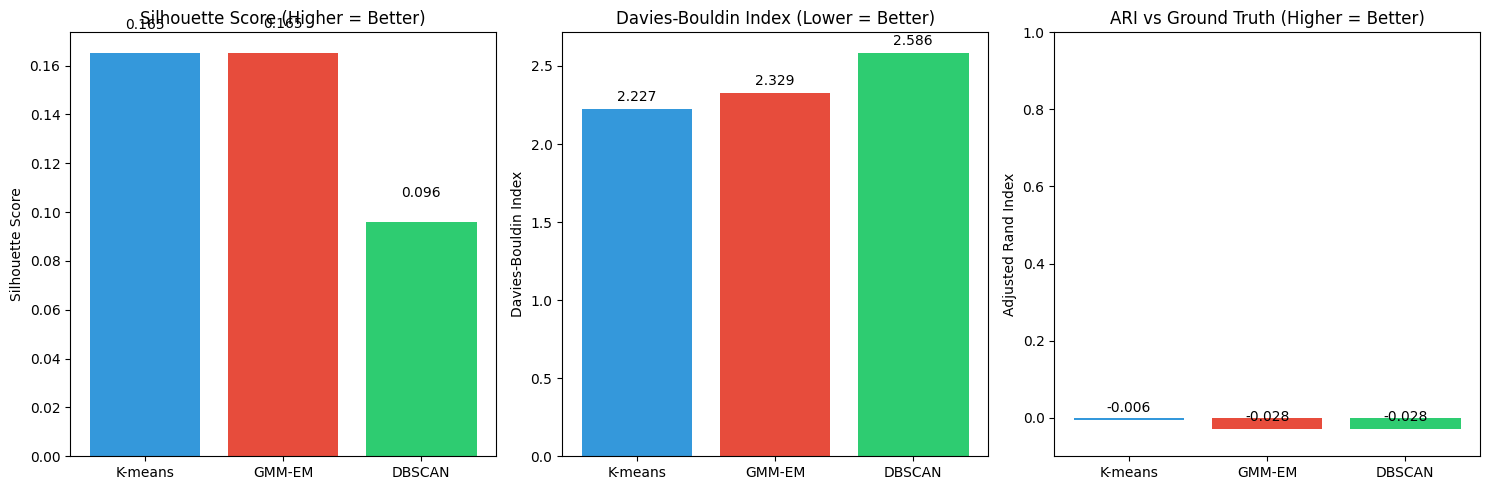
\includegraphics[width=\linewidth]{figures/metrics_comparison.png}
  \caption{So sánh các chỉ số, trích nguyên từ notebook.
  Silhouette và ARI càng cao càng tốt; Davies--Bouldin càng thấp càng tốt.
  Nhãn trên các cột được làm tròn đến ba chữ số thập phân.}
  \label{fig:ev_metrics}
\end{figure}

Hình~\ref{fig:ev_metrics} cho thấy Silhouette của K-means và GMM gần như
bằng nhau; cả hai nhãn làm tròn thành 0.165. Khoảng hiển thị lớn của trục
ARI khiến các giá trị âm khó phân biệt, nên Bảng~\ref{tab:ev_metrics}
phù hợp hơn để đối chiếu chính xác. Cả ba ARI đều âm và gần 0:
các phân hoạch chưa tái hiện được phân nhóm theo nhãn mua xe điện dưới
thước đo này, ngay cả khi xác suất thuộc thành phần cao. Không thể
diễn giải trực tiếp mã cụm thành nhãn dự đoán của \texttt{Will\_Buy\_EV}.

DBSCAN tìm được tám cụm và gán 1.385 quan sát là nhiễu, tương ứng 9.2\%
theo output. Trên các điểm giữ lại, Silhouette đạt 0.0961 và
Davies--Bouldin đạt 2.5860, kém thuận lợi hơn về mặt số học so với hai
phương pháp còn lại. Tuy nhiên, số cụm và tập mẫu đánh giá đều khác nhau;
ngay cả ARI cũng dùng nhãn mục tiêu sau khi lọc nhiễu. Bảng vì vậy phản ánh
từng cấu hình và tập con tương ứng, chưa phải so sánh có kiểm soát trên
cùng tập quan sát. Nhãn nhiễu phụ thuộc tham số mật độ, chưa đủ để kết luận
các bản ghi đó sai hoặc bất thường về mặt thực tiễn.

\begin{figure}[H]
  \centering
  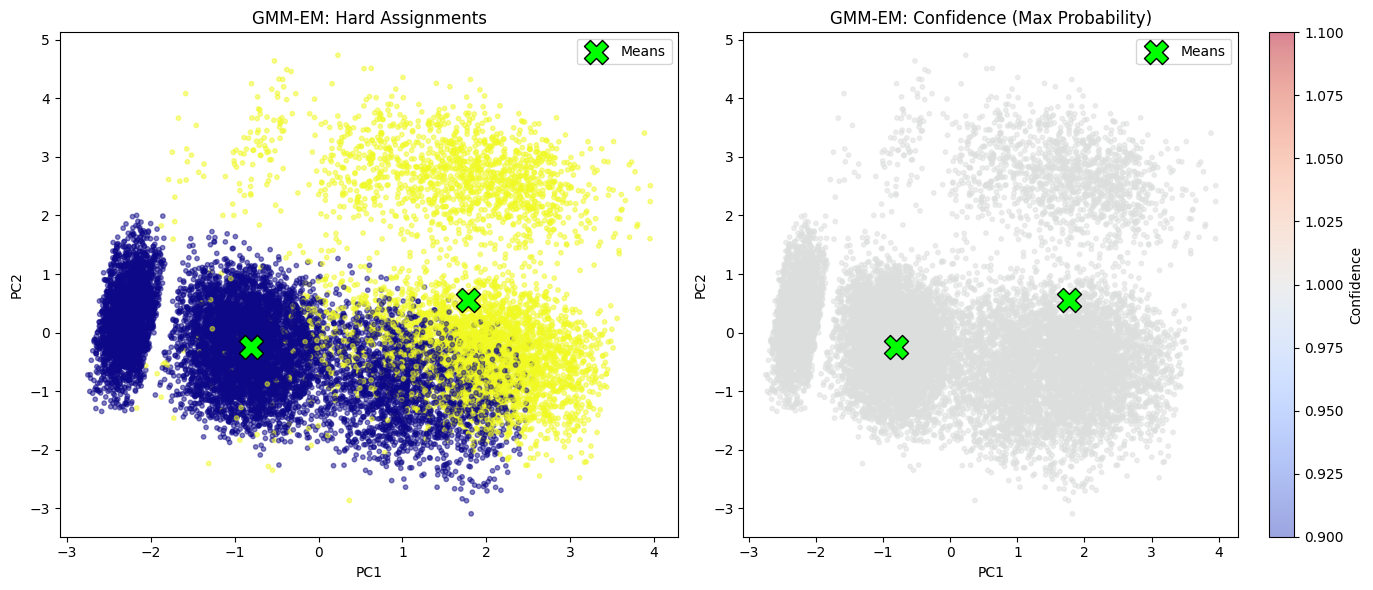
\includegraphics[width=\linewidth]{figures/gmm_clusters.png}
  \caption{Kết quả GMM gốc trên hai thành phần chính: gán cụm cứng (trái)
  và xác suất thuộc thành phần lớn nhất (phải). Dấu chéo xanh lá biểu diễn
  trung bình thành phần sau phép chiếu. PCA giữ lại 30.6\% phương sai.
  Vạch trên 1 của thang màu là hệ quả hiển thị, không phải xác suất hợp lệ.}
  \label{fig:ev_gmm}
\end{figure}

Trong Hình~\ref{fig:ev_gmm}, hai nhóm bên trái có vùng chồng lấn trên phép
chiếu, còn màu bên phải gần như đồng nhất quanh xác suất lớn nhất bằng 1.
Thang màu tự mở rộng từ khoảng 0.9 đến 1.1; vạch trên 1 không biểu thị
xác suất hậu nghiệm hợp lệ. Các xác suất được tính trong không gian
13 chiều, nên chồng lấn trên hình hai chiều không đồng nghĩa với gán cụm
thiếu chắc chắn. Xác suất thuộc thành phần cao cũng chưa chứng minh
các thành phần tương ứng với hành vi mua xe điện hoặc phân khúc có ý nghĩa.

\subsection{Các phát hiện chính}
GMM và K-means có Silhouette gần như bằng nhau tại cấu hình hai thành phần,
trong khi K-means có Davies--Bouldin tốt hơn. Chưa có cơ sở khẳng định GMM
vượt trội đáng kể. DBSCAN tạo phân hoạch nhiều cụm hơn cùng một tập nhiễu,
nhưng các chỉ số nội tại kém thuận lợi hơn chỉ áp dụng cho những điểm giữ
lại tại bán kính và ngưỡng mật độ đã chọn.

Thông tin bổ sung của GMM là vectơ xác suất thuộc thành phần; với hai thành
phần, $\responsibility_{i1}+\responsibility_{i2}=1$. Phần tử lớn nhất
cho biết mức độ mô hình nghiêng về một thành phần khi gán quan sát.
Về nguyên tắc, thông tin này giúp thể hiện trường hợp khó gán cụm,
dù biểu đồ trong lần chạy đã lưu cho thấy rất ít biến thiên.
Đây là xác suất thuộc thành phần ẩn với điều kiện biết đặc trưng và mô hình
đã khớp; không phải xác suất một người sẽ mua xe điện.
Các ARI âm gần 0 càng cho thấy cần phân biệt hai cách diễn giải này.

Hình \texttt{gmm\_uncertainty.png} không được đưa vào báo cáo vì thang màu
diễn giải ngược đại lượng được vẽ. Mã nguồn tính
\[
 u_i=1-2\left|\responsibility_{i1}-0.5\right|.
\]
Với hai thành phần, $u_i=1$ ứng với hai xác suất bằng nhau, tức bất định
gán cụm cao nhất; $u_i=0$ ứng với gán cụm hoàn toàn chắc chắn theo mô hình.
Tuy nhiên, thang màu lại gọi 1 là \emph{certain} (chắc chắn).
Dòng \emph{certainty $>80\%$} kiểm tra $u_i>0.6$, còn dòng
\emph{certainty $<20\%$} kiểm tra $u_i<0.2$; không thể dùng tên các dòng này
để kết luận về mức chắc chắn. Hai output tương ứng, 0.0\% và 100.0\%,
là tỉ lệ đã làm tròn của các điều kiện về bất định trên. Chúng phù hợp với
việc phần lớn quan sát được gán thành phần rõ ràng, chưa cho thấy tình trạng
khó gán cụm xảy ra phổ biến.

Một số giới hạn cần được cân nhắc. Mã hóa phân loại bằng số nguyên tạo ra
thứ tự và khoảng cách có thể không có ý nghĩa thực tiễn; chuẩn hóa không
loại bỏ tác động này. PCA bỏ qua 69.4\% phương sai, hạn chế kết luận từ
hình ảnh. Kết quả chỉ dựa trên một mẫu và một cấu hình cuối có hạt giống
cố định cho mỗi phương pháp, dù K-means và GMM có nhiều lần khởi tạo nội bộ.
Số cụm bằng hai, dạng hiệp phương sai và tham số DBSCAN đều có thể ảnh hưởng
kết quả; khảo sát K-means thực tế ưu tiên ba cụm theo Silhouette.
Notebook cũng không có đánh giá trên tập kiểm tra độc lập, so sánh thời gian
hay phân tích qua nhiều lần chạy. Kết luận về khả năng dự đoán, ưu thế
tính toán và độ ổn định cần được kiểm chứng bằng thí nghiệm bổ sung.

\clearpage

\input{chapters/07_conclusion}
\clearpage

% ------------------------------------------------------------
%  Tài liệu tham khảo
% ------------------------------------------------------------
\printbibliography[heading=bibintoc, title={Tài liệu tham khảo}]

\end{document}
